\documentclass[12px]{article}
\usepackage[utf8]{inputenc}

\usepackage{color}
\usepackage{listings}
\usepackage{polski}
\usepackage[utf8]{inputenc}
\usepackage{geometry}
\usepackage{graphicx}

\graphicspath{ {./obrazki/} }

\usepackage{hyperref}
\hypersetup{
    colorlinks=true,
    linkcolor=black,
    filecolor=magenta,      
    urlcolor=blue,
    pdftitle={Projekt Zaliczeniowy - Bazy Danych - Semestr 5},
    bookmarks=true,
    bookmarksopen=true,
    pdfpagemode=FullScreen,
    breaklinks=true,
}
\urlstyle{same}

\geometry{a4paper, margin=0.85in}

\title{Projekt Zaliczeniowy - Bazy Danych - Semestr 5}
\author{Krystian Duma Grupa - Z501 - Nr. Albumu 7763}
\date{23 Grudzień 2018}

%\definecolor{mygreen}{rgb}{0,0.6,0}
%\definecolor{mygray}{rgb}{0.5,0.5,0.5}
%\definecolor{mymauve}{rgb}{0.58,0,0.82}

\lstset{ 
%  basicstyle=\scriptsize,        % the size of the fonts that are used for the code
%  breakatwhitespace=false,         % sets if automatic breaks should only happen at whitespace
%  breaklines=true,                 % sets automatic line breaking
%  captionpos=t,                    % sets the caption-position to bottom
%  commentstyle=\color{mygreen},    % comment style
%  extendedchars=true,              % lets you use non-ASCII characters; for 8-bits encodings only, does not work with UTF-8
%  frame=single,	                   % adds a frame around the code
%%  keepspaces=true,                 % keeps spaces in text, useful for keeping indentation of code (possibly needs columns=flexible)
%  keywordstyle=\color{blue},       % keyword style
%%  language=Octave,                 % the language of the code
%  numbers=left,                    % where to put the line-numbers; possible values are (none, left, right)
%  numbersep=5pt,                   % how far the line-numbers are from the code
%  numberstyle=\tiny\color{mygray}, % the style that is used for the line-numbers
%  rulecolor=\color{black},         % if not set, the frame-color may be changed on line-breaks within not-black text (e.g. comments (green here))
%  showspaces=false,                % show spaces everywhere adding particular underscores; it overrides 'showstringspaces'
%  showstringspaces=false,          % underline spaces within strings only
%  showtabs=false,                  % show tabs within strings adding particular underscores
%  stepnumber=1,                    % the step between two line-numbers. If it's 1, each line will be numbered
%  stringstyle=\color{mymauve},     % string literal style
%  tabsize=2,	                   % sets default tabsize to 2 spaces
%  title=\lstname                   % show the filename of files included with \lstinputlisting; also try caption instead of title
}

\definecolor{codegreen}{rgb}{0,0.6,0}
\definecolor{codegray}{rgb}{0.5,0.5,0.5}
\definecolor{codepurple}{rgb}{0.58,0,0.82}
\definecolor{backcolour}{rgb}{0.95,0.95,0.92}
 
\lstdefinestyle{mystyle}{
    backgroundcolor=\color{backcolour},   
    commentstyle=\color{codegreen},
    keywordstyle=\color{magenta},
    numberstyle=\tiny\color{codegray},
    stringstyle=\color{codepurple},
    basicstyle=\footnotesize,
    breakatwhitespace=false,         
    breaklines=true,                 
    captionpos=b,                    
    keepspaces=true,                 
    numbers=left,                    
    numbersep=5pt,                  
    showspaces=false,                
    showstringspaces=false,
    showtabs=false,                  
    tabsize=2
}

\lstset{style=mystyle}
\lstMakeShortInline[columns=fixed, language=SQL]|

\begin{document}

\maketitle

\tableofcontents

\newpage

\section{Krótki opis słowny projektu}
Projekt systemu zawiera założenia do bazy danych przechowującej informacje potrzebne



\section{Założenia do projektu}

Przyjęte zostały następujące założenia do projektu
\begin{enumerate}

	\item Podstawowe Obiekty
	\begin{itemize}
		\item \texttt{Obiekt} - obiekt najmu - np. konkretny dom lub mieszkanie,
		\item \texttt{Użytkownik} - osoba wynajmująca mieszkanie lub dom,
%		\item \texttt{Miasto} oraz \texttt{Dzielnica} - kategorie "geograficzne",
%		\item \texttt{Kategoria} - kategorie "nie-geograficzne" (np. \textsl{Dom}, \textsl{Willa} lub \textsl{Kawalerka}).
	\end{itemize}

	\item Przechowywane zadania (transakcje)
	\begin{itemize}
		\item \texttt{Najem} - transakcja związana z wynajęciem \texttt{Obiektu} przez \texttt{Użytkownika}.
	\end{itemize}
	
	\item Szczegóły opisu
	\begin{itemize}
		\item \texttt{Użytkownik} - potrzeba przechowania informacji: nazwisko klienta, imię klienta, wiek klienta, adres zamieszkania klienta, telefon klienta, płeć klienta oraz login używany do logowania do bazy danych.

		\item \texttt{Obiekt} - potrzeba przechowania informacji: nazwa własna obiektu, adres obiektu, dzienna stawka najmu obiektu, kategoria obiektu, obecny status najmu obiektu (informacja czy dany obiekt jest obecnie wolny lub zajęty), opis obiektu oraz inne atrybuty odpowiednie dla zgromadzonych obiektów.
		\begin{itemize}
			\item Każdy obiekt może znajdować się w wielu różnych kategoriach,
			\item Dla uproszczenia inne atrybuty będą znajdować się w opisie danego obiektu.
		\end{itemize}
		
		\item \texttt{Najem} - potrzeba przechowania informacji: użytkownika-najemca, wynajmowany obiekt, data rozpoczęcia najmu, data zakończenia najmu, koszt najmu.
		\begin{itemize}
			\item Najem to transakcja tylko jednego \texttt{Użytkownika} i tylko jednego \texttt{Obiektu},
			\item Dla uproszczenia najem jest liczony od godziny 00:00 do godziny 23:59,
			\item Jeden \texttt{Obiekt} może być w danym czasie wynajęty tylko jednemu użytkownikowi.
		\end{itemize}
		
	\end{itemize}

	\item Użytkownicy i Uprawnienia
		\begin{itemize}
			\item Administrator ma dostęp do danych wszystkich użytkowników,
			\item Każdy \texttt{Użytkownik} ma założone oddzielne konto serwera SQL,
			\item Użytkownicy nie widzą danych oraz wypożyczeń innych użytkowników.
		\end{itemize}

\end{enumerate}

\section{Środowisko Projektowe}

Środowiskiem uruchomieniowym jest baza danych \href{https://www.microsoft.com/pl-pl/sql-server/sql-server-2017}{Microsoft SQL Server 2017} uruchomiona w kontenerze \href{https://www.docker.com}{Docker}'a. Jako obraz bazowy został wybrany obraz \href{https://hub.docker.com/r/microsoft/mssql-server}{mcr.microsoft.com/mssql/server:2017-latest-ubuntu} który zawiera najaktualniejszą obecnie wersję \href{https://www.microsoft.com/pl-pl/sql-server/sql-server-2017}{Microsoft SQL Server 2017} uruchomioną na systemie Linux - \href{https://www.ubuntu.com/server}{Ubuntu Server}. Do obrazu zostały doinstalowane dodatkowe narzędzia umożliwiające przygotowanie plików wyjściowych: tego dokumentu pdf (\href{https://pl.wikipedia.org/wiki/LaTeX}{\LaTeX}) oraz skryptów tworzących i usuwających obiekty z bazy (\href{http://www.php.net}{PHP}).


Jako aplikację służącą do łączenia się i wykonywania poleceń wykorzystane zostały aplikacje: 

\begin{itemize}
\item Dołączona do \href{https://www.microsoft.com/pl-pl/sql-server/sql-server-2017}{SQL Server}'a aplikacja wiersza poleceń - \href{https://docs.microsoft.com/en-us/sql/tools/sqlcmd-utility?view=sql-server-2017}{sqlcmd}
\item Środowisko IDE od czeskiej firmy \href{https://www.jetbrains.com/}{JetBrains} - \href{https://www.jetbrains.com/datagrip/}{DataGrip}
\item Środowisko IDE od \href{https://microsoft.com/}{Microsoft}'u - \href{https://docs.microsoft.com/en-us/sql/ssms/download-sql-server-management-studio-ssms?view=sql-server-2017}{SQL Server Management Studio (SSMS)}
\end{itemize}

\section{Model fizyczny bazy danych}


\section{Skrypt tworzący obiekty w bazie danych}

\subsection{Model wersjonowania bazy danych}

Jak można zauważyć na Rysunku \ref{fig:diagram}, w bazie danych znajduje się jedna dodatkowa tabela \texttt{db\_status} z jednym polem \texttt{version} - służy ona do przechowywania wersji bazy danych.
Każda operacja w \href{run:skrypt_tworzacy_obiekty_w_bazie_danych.sql}{skrypcie tworzącym} sprawdza i porównuje obecną oraz oczekiwaną wersję dla danej operacji. 
Dzięki temu zabiegowi nie będzie można uruchomić danej operacji dla jednej bazy danych wielokrotnie. Dodatkowo aktualizacja istniejącej bazy danych do najnowszej wersji będzie uproszczona - wystarczy uruchomić najnowszą wersję skryptu, a wykonane zostaną tylko nowe operacje dodane od ostatniego uruchomienia skryptu instalacyjnego.
Każda operacja jest opakowana zgodnie z szablonem z listingu \ref{lst:versioning}.

\begin{lstlisting}[language=SQL, caption=Szablon kodu wersjonowanego, label={lst:versioning}]
PRINT 'Wersja X: ''<<< OPIS OPERACJI >>>'''
IF EXISTS(SELECT * FROM sys.tables WHERE name = N'db_status')
  BEGIN
    IF EXISTS(SELECT * FROM db_status WHERE version = X)
      BEGIN
		
		<<< MIEJSCE NA KOD >>>        
            
        UPDATE db_status SET version = 1 WHERE version = X;
        PRINT 'Wersja X: Migracja zostala zainstalowana pomyslnie - teraz baza jest w wersji X';
      END
    ELSE
      BEGIN
        IF EXISTS(SELECT * FROM db_status WHERE version < X)
          BEGIN
            RAISERROR ('Wersja X: Baza danych jest w za niskiej wersji (wymagana jest wersja X) aby zainstalowac migracje', 11, 2);
          END
        ELSE
          BEGIN
            PRINT 'Wersja X: Migracja już zostala zainstalowana wczesniej';
          END
      END
  END
ELSE
  BEGIN
    RAISERROR ('Wersja X: Nie znaleziono tabeli wersjonowania bazy danych', 11, 1);
  END
\end{lstlisting}

Dodatkowo w przypadku wystąpienia jakichkolwiek błędów jest przewidziana procedura ich łapania - na listingu \ref{lst:catch} widzimy zawartość bloku \texttt{CATCH} skryptu instalacyjnego. Skrypt został przygotowany w taki sposób aby w przypadku wystąpienia błędu przerywał działanie\footnote{Aby wywołanie funkcji \href{https://docs.microsoft.com/en-us/sql/t-sql/language-elements/raiserror-transact-sql?view=sql-server-2017}{\texttt{RAISERROR}} przekazało kontrolę do bloku \texttt{CATCH}, parametr \texttt{severity} musi mieć wartość z zakresu od \texttt{11} do \texttt{19}. Wartości poniżej nie powodują przerwania skryptu, a wartości powyżej terminują połączenie z bazą danych.} i przechodził od razu do bloku \texttt{CATCH}.

\begin{lstlisting}[language=SQL, caption=Blok CATCH w skrypcie tworzącym, label={lst:catch}]
BEGIN CATCH

  SELECT
    ERROR_NUMBER() AS ErrorNumber,
    ERROR_SEVERITY() AS ErrorSeverity,
    ERROR_STATE() AS ErrorState,
    ERROR_PROCEDURE() AS ErrorProcedure,
    ERROR_LINE() AS ErrorLine,
    ERROR_MESSAGE() AS ErrorMessage;

END CATCH;
\end{lstlisting}


\subsection{Wynik uruchomienia całego skryptu tworzącego obiekty w trybie wsadowym}

Jak widać na listingu \ref{lst:create-objects}, skrypt podaje bardzo dokładne informacje na temat aktualnie wykonywanej operacji. W większości przypadków wystąpienia ciągu tekstowego \texttt{(1 rows affected )}, następuje zmiana aktualnej wersji bazy danych w tabeli wersjonowania - \texttt{db\_status}.

\lstinputlisting[caption=Wynik uruchomienia całego skryptu tworzącego obiekty w trybie wsadowym, label={lst:create-objects}]{../Logs/skrypt_tworzacy_obiekty_w_bazie_danych.sql-second-run.log}

\newpage

\subsection{Tabele}

Wszystkie tabele są tworzone przez 13 skryptów \texttt{SQL}:
\begin{itemize}
	\item \href{run:Sources/SQL/1. Tabele/001_Utworzenie_tabeli_z_miastami.sql}{Utworzenie tabeli z miastami}
	\item \href{run:Sources/SQL/1. Tabele/002_Utworzenie_tabeli_z_dzielnicami.sql}{Utworzenie tabeli z dzielnicami}
	\item \href{run:Sources/SQL/1. Tabele/003_Utworzenie_relacji_pomiedzy_miastami_a_dzielnicami.sql}{Utworzenie relacji pomiedzy miastami a dzielnicami}
	\item \href{run:Sources/SQL/1. Tabele/004_Utworzenie_tabeli_z_kategoriami.sql}{Utworzenie tabeli z kategoriami}
	\item \href{run:Sources/SQL/1. Tabele/005_Utworzenie_tabeli_z_obiektami.sql}{Utworzenie tabeli z obiektami}
	\item \href{run:Sources/SQL/1. Tabele/006_Utworzenie_relacji_pomiedzy_dzielnicami_a_obiektami.sql}{Utworzenie relacji pomiedzy dzielnicami a obiektami}
	\item \href{run:Sources/SQL/1. Tabele/007_Utworzenie_relacji_pomiedzy_kategoriami_a_obiektami.sql}{Utworzenie relacji pomiedzy kategoriami a obiektami}
	\item \href{run:Sources/SQL/1. Tabele/008_Utworzenie_tabeli_z_uzytkownikami.sql}{Utworzenie tabeli z uzytkownikami}
	\item \href{run:Sources/SQL/1. Tabele/009_Utworzenie_tabeli_z_najmami.sql}{Utworzenie tabeli z najmami}
	\item \href{run:Sources/SQL/1. Tabele/010_Utworzenie_indeksu_unikatowego_w_tabeli_z_najemcami.sql}{Utworzenie indeksu unikatowego w tabeli z najemcami}
	\item \href{run:Sources/SQL/1. Tabele/011_Utworzenie_relacji_pomiedzy_uzytkownikami_a_najmami.sql}{Utworzenie relacji pomiedzy uzytkownikami a najmami}
	\item \href{run:Sources/SQL/1. Tabele/012_Utworzenie_relacji_pomiedzy_obiektami_a_najmami.sql}{Utworzenie relacji pomiedzy obiektami a najmami}
	\item \href{run:Sources/SQL/1. Tabele/013_Utworzenie_indeksu_unikatowego_w_tabeli_z_uzytkownikami}{Utworzenie indeksu unikatowego w tabeli z uzytkownikami}
\end{itemize}

Tworzenie relacji pomiędzy tabelami oraz indeksów zostało oddzielone od operacji tworzenia poszczególnych tabel - celem tego działania jest lepsza organizacja skryptów. Dodatkowo oddzielając te operacje, w przypadku wystąpienia jakiegoś błędu jesteśmy w stanie określić co i gdzie się "wysypało".

\subsubsection{Utworzenie tabeli z obiektami}

Ponieważ polecenia \href{https://docs.microsoft.com/pl-pl/sql/t-sql/statements/create-default-transact-sql?view=sql-server-2017}{\texttt{CREATE DEFAULT}} oraz \href{https://docs.microsoft.com/pl-pl/sql/t-sql/statements/create-rule-transact-sql?view=sql-server-2017}{\texttt{CREATE RULE}} zostały zdeprecjonowane i w kolejnych wersjach SQL Serwera prawdopodobnie zostaną usunięte zdecydowałem się umieścić wartości domyślne oraz reguły sprawdzające w definicjach konkretnych tabel.

W wyniku projektowania zostało dodatkowo ustalone że \texttt{dzienna\_stawka\_najmu} musi być większa od 0.

Status obiektu znajdujący się w polu \texttt{obecnie\_wynajete} może przyjmować dwie wartości \texttt{T} oraz \texttt{N} - odpowiednio dla obiekty wynajętego oraz wolnego.

\begin{lstlisting}[language=SQL, caption={Skrypt tworzący tabelę \texttt{obiekty}}, label={lst:table-objects}]
CREATE TABLE obiekty (
  id INT PRIMARY KEY NOT NULL IDENTITY (1, 1),

  dzielnica_id INT NOT NULL,
  kategoria_id INT NOT NULL,

  nazwa VARCHAR(150) NOT NULL,
  adres VARCHAR(150) NOT NULL DEFAULT 'Brak Danych',
  dzienna_stawka_najmu DECIMAL(10, 2) NOT NULL CHECK (dzienna_stawka_najmu > 0),

  obecnie_wynajete CHAR(1) NOT NULL DEFAULT 'N' CHECK (obecnie_wynajete IN ('T', 'N')),
);
\end{lstlisting}

\begin{figure}[h]
	\centering
    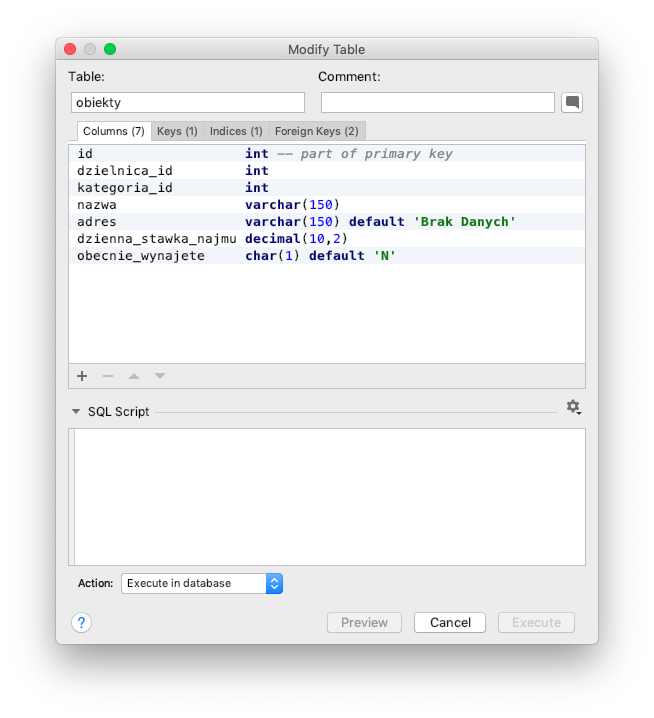
\includegraphics[width=0.4\textwidth]{objects}
	\caption{Tabela \texttt{obiekty} wyświetlona w programie \href{https://www.jetbrains.com/datagrip/}{DataGrip}}
	\label{fig:objects}
\end{figure}

\subsubsection{Utworzenie tabeli z najmami}

Przyjmujemy że domyślną datą rozpoczęcia najmu jest data jego dodania do bazy.

\begin{lstlisting}[language=SQL, caption={Skrypt tworzący tabelę \texttt{obiekty}}, label={lst:table-najmy}]
CREATE TABLE najmy (
  id INT PRIMARY KEY NOT NULL IDENTITY (1, 1),

  uzytkownik_id INT NOT NULL,
  obiekt_id INT NOT NULL,

  data_rozpoczecia DATE NOT NULL DEFAULT getdate(),
  data_zakonczenia DATE NULL,
  koszt DECIMAL(15, 2) NULL,
);
\end{lstlisting}

\begin{figure}[h]
	\centering
    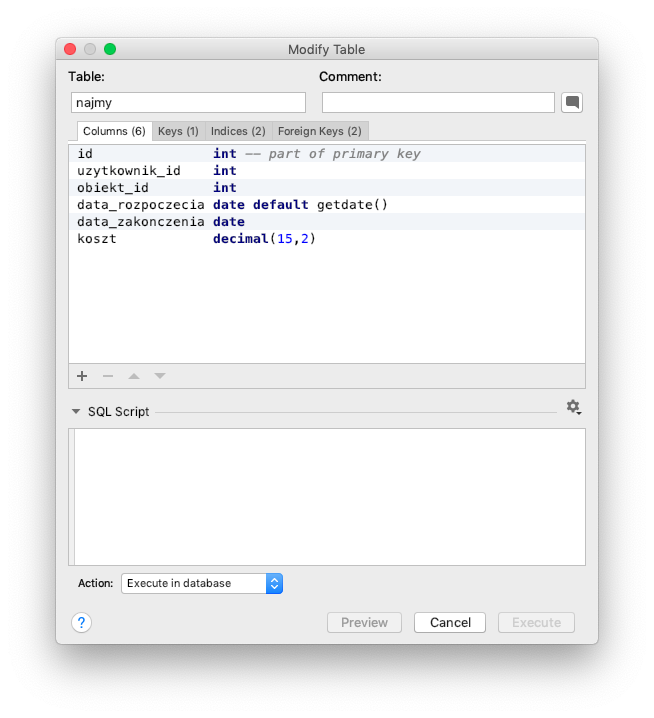
\includegraphics[width=0.4\textwidth]{najmy}
	\caption{Tabela \texttt{najmy} wyświetlona w programie \href{https://www.jetbrains.com/datagrip/}{DataGrip}}
	\label{fig:najmy}
\end{figure}

\newpage

\subsection{Widoki}

Zostało stworzone kilka widoków:
\begin{itemize}
	\item \href{run:Sources/SQL/2. Widoki/014_Utworzenie_widoku_z_lista_wszystkich_najmow.sql}{\texttt{lista\_najmow} - Lista wszystkich najmów}
	\item \href{run:Sources/SQL/2. Widoki/015_Utworzenie_widoku_z_lista_popularnosci_obiektow.sql}{\texttt{lista\_popularnosci\_obiektow} - Lista obiektów wraz z ilością (popularnoscią) ich najmów}
	\item \href{run:Sources/SQL/2. Widoki/016_Utworzenie_widoku_z_lista_niewynajmowanych_obiektow.sql}{\texttt{lista\_niepopularnych\_obiektow} - Lista obiektów które nie zostały nigdy wynajęte}
\end{itemize}

\subsubsection{\texttt{lista\_najmow} - Lista wszystkich najmów}

Widok ten zwraca listę wszystkich najmów, wraz z następującymi polami:
\begin{itemize}
	\item nazwisko
	\item imie
	\item datę rozpoczecia najmu
	\item datę zakonczenia najmu
	\item nazwę wynajmowanego obiektu
	\item całkowity koszt najmu
\end{itemize}

\begin{figure}[h]
	\centering
    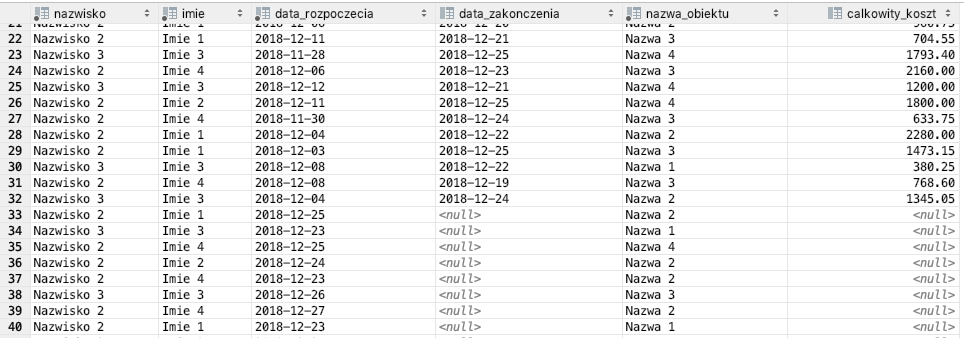
\includegraphics[width=0.9\textwidth]{lista_najmow}
	\caption{Wyświetlony widok \texttt{lista\_najmow}}
	\label{fig:lista_najmow}
\end{figure}

\begin{lstlisting}[language=SQL, caption={Skrypt tworzący widok \texttt{lista\_najmow}}, label={lst:view-lista_najmow}]
CREATE VIEW lista_najmow
  AS
    SELECT nazwisko, imie, data_rozpoczecia, data_zakonczenia, nazwa nazwa_obiektu, koszt calkowity_koszt
        FROM najmy n
        JOIN uzytkownicy u on n.uzytkownik_id = u.id
        JOIN obiekty o on n.obiekt_id = o.id;
\end{lstlisting}



\subsubsection{\texttt{lista\_niepopularnych\_obiektow} - Lista obiektów które nie zostały nigdy wynajęte}

Widok ten zwraca listę obiektów które nie zostały nigdy, prze nikogo, wynajęte, wraz z następującymi polami:
\begin{itemize}
	\item nazwę obiektu
	\item adres obiektu
\end{itemize}

Widok ten korzysta z innego (nieopisanego w tym dokumencie) widoku - \texttt{lista\_popularnosci\_obiektow}.

\begin{figure}[h]
	\centering
    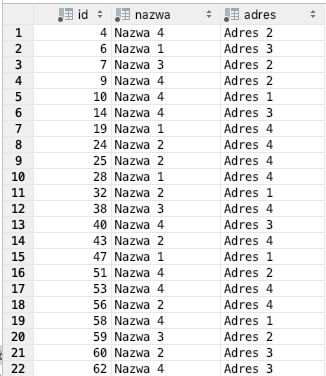
\includegraphics[width=0.4\textwidth]{lista_niepopularnych_obiektow}
	\caption{Wyświetlony widok \texttt{lista\_niepopularnych\_obiektow}}
	\label{fig:lista_niepopularnych_obiektow}
\end{figure}

\begin{lstlisting}[language=SQL, caption={Skrypt tworzący widok \texttt{lista\_niepopularnych\_obiektow}}, label={lst:view-lista_niepopularnych_obiektow}]
CREATE VIEW lista_niepopularnych_obiektow
  AS
    SELECT id, nazwa, adres
      FROM lista_popularnosci_obiektow
      GROUP BY id, nazwa, adres
      HAVING SUM(liczba_najmow) = 0;
\end{lstlisting}

\newpage

\subsection{Funkcje Skalarne i Tabelarne}

Zostały stworzone następujące funkcje:
\begin{itemize}
	\item \href{run:Sources/SQL/3. Funkcje Skalarne/017_Utworzenie_funkcji_wyliczajacej_koszt_najmu_obiektu.sql}{\texttt{koszt\_najmu\_obiektu} - Funkcja obliczająca koszt najmu wskazanego obiektu}
	\item \href{run:Sources/SQL/3. Funkcje Skalarne/018_Utworzenie_funkcji_wyliczajacej_koszt_konkretnego_najmu.sql}{\texttt{koszt\_najmu} - Funkcja obliczająca koszt konkretnego najmu}
	\item \href{run:Sources/SQL/3. Funkcje Skalarne/020_Utworzenie_funkcji_wyswietlajacej_adresowke_uzytkownika.sql}{\texttt{adresowka} - Funkcja generująca etykietę adresową dla użytkownika}
	\item \href{run:Sources/SQL/4. Funkcje Tabelarne/021_Utworzenie_funkcji_wyswietlajacej_spozniajacych_sie_uzytkownikow.sql}{\texttt{opoznieni} - Funkcja generująca etykiety dla użytkowników którzy coś wynajęli ale jeszcze nie oddali}
\end{itemize}

\subsubsection{\texttt{koszt\_najmu\_obiektu} - Funkcja obliczająca koszt najmu wskazanego obiektu}

`koszt_najmu_obiektu (@obiekt_id INT, @liczba_dni INT)` - Funkcja ta oblicza koszt najmu obiektu wskazanego w parametrze `@obiekt_id` przez liczbę dni określoną w parametrze `@liczba_dni`, zwracana wartość ma typ `DECIMAL(15, 2)` który jest kompatybilny z typem kolumny \texttt{koszt} w tabeli \texttt{najmy}. Funkcja ta została wydzielona w celu uniknięcia duplikacji kodu w funkcji skalarnej \texttt{koszt\_najmu} z listingu \ref{lst:function-koszt_najmu} oraz w funkcji tabelarnej \texttt{opoznieni} z listingu \ref{lst:function-opoznieni} (strona \pageref{lst:function-opoznieni}).

\begin{lstlisting}[language=SQL, caption={Skrypt tworzący funkcję skalarną \texttt{koszt\_najmu\_obiektu}}, label={lst:function-koszt_najmu_obiektu}]
CREATE FUNCTION koszt_najmu_obiektu (@obiekt_id INT, @liczba_dni INT)
  RETURNS DECIMAL(15, 2)
  AS
  BEGIN
    DECLARE @dzienna_stawka DECIMAL(10,2);

    SELECT @dzienna_stawka = dzienna_stawka_najmu
      FROM obiekty o
      WHERE id = @obiekt_id;

    RETURN @liczba_dni*@dzienna_stawka;
  END
\end{lstlisting}

\subsubsection{\texttt{koszt\_najmu} - Funkcja obliczająca koszt danego najmu}

`koszt_najmu (@najem_id INT)` - Funkcja ta oblicza koszt konkretnego najmu wskazanego w parametrze `@najem_id`, zwracana wartość ma taki sam typ jak funkcja \texttt{koszt\_najmu\_obiektu} która jest wywoływana - czyli `DECIMAL(15, 2)` który jest kompatybilny z typem kolumny \texttt{koszt} w tabeli \texttt{najmy}. Przykład wykorzystania tej funkcji jest w triggerze z listingu \ref{lst:trigger-wylicz_koszt_najmu} (strona \pageref{lst:trigger-wylicz_koszt_najmu}).

\begin{lstlisting}[language=SQL, caption={Skrypt tworzący funkcję skalarną \texttt{koszt\_najmu}}, label={lst:function-koszt_najmu}]
CREATE FUNCTION koszt_najmu (@najem_id INT)
  RETURNS DECIMAL(15, 2)
  AS
  BEGIN
    DECLARE @koszt DECIMAL(15, 2);
    DECLARE @liczba_dni INT;
    DECLARE @obiekt_id INT;
    DECLARE @data_rozpoczecia DATE;
    DECLARE @data_zakonczenia DATE;

    SELECT @data_rozpoczecia = n.data_rozpoczecia,
           @data_zakonczenia = n.data_zakonczenia,
           @obiekt_id = o.id
      FROM najmy n
      JOIN obiekty o on n.obiekt_id = o.id
      WHERE n.id = @najem_id;

    IF @data_zakonczenia IS NULL
      RETURN NULL;

    SELECT @liczba_dni = (1+DATEDIFF(DAY, @data_rozpoczecia, @data_zakonczenia));

    SELECT @koszt = dbo.koszt_najmu_obiektu(@obiekt_id, @liczba_dni);

    RETURN @koszt;
  END
\end{lstlisting}

\subsubsection{\texttt{adresowka} - Funkcja generująca etykietę adresową dla użytkownika}

`adresowka (@uzytkownik_id INT)` - Funkcja ta generuje zawartość etykiety adresowej dla użytkownika wskazanego w parametrze `@uzytkownik_id`, zwracana wartość ma typ `VARCHAR(333)`\footnote{Rozmiar pola bierze się z sumy długości użytych pól (\texttt{nazwisko} i \texttt{imie} po 75 znaków, \texttt{telefon} 30 znaków,\texttt{adres} 150 znaków) oraz znaków dodanych (jedna spacja i dwa znaki nowej lini - \texttt{CHAR(13)}) - jest to najdłuższy możliwy wynik tej funkcji.}. Przykład wykorzystania tej funkcji jest w funkcji tabelarnej z listingu \ref{lst:function-opoznieni}.

\begin{lstlisting}[language=SQL, caption={Skrypt tworzący funkcję skalarną \texttt{adresowka}}, label={lst:function-adresowka}]
CREATE FUNCTION adresowka (@uzytkownik_id INT)
  RETURNS VARCHAR(333) -- 75+75+150+30+3 = 333 - suma długości łączonych pól
  AS
  BEGIN
    DECLARE @adresowka VARCHAR(330);

    SELECT @adresowka = nazwisko + ' ' + imie + CHAR(13) + telefon + CHAR(13) + adres
      FROM uzytkownicy
      WHERE id = @uzytkownik_id;

    RETURN @adresowka;
  END
\end{lstlisting}

\subsubsection{\texttt{opoznieni} - Funkcja generująca etykiety dla użytkowników którzy coś wynajęli ale jeszcze nie oddali}

`opoznieni (@liczba_dni INT)` - Funkcja ta generuje listę obiektów wraz z najemcami, które zostały wynajęte co najmniej liczbę dni wcześniej określoną parametrem `@liczba_dni`. Funkcja ta zwraca tabelę składającą się z identyfikatora najmu, nazwy wynajętego obiektu, liczby dni od rozpoczęcia najmu, szacunkowego kosztu tego najmu na dzień bieżący oraz etykiety adresowej do najemcy.

\begin{figure}[h]
	\centering
    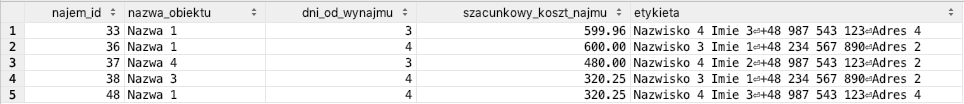
\includegraphics[width=0.8\textwidth]{opoznieni}
	\caption{Uruchomiona funkcja \texttt{opoznieni} z parametrem \texttt{@liczba\_dni} równym 3}
	\label{fig:opoznieni}
\end{figure}

\begin{lstlisting}[language=SQL, caption={Skrypt tworzący funkcję tabelarną \texttt{opoznieni}}, label={lst:function-opoznieni}]
CREATE FUNCTION opoznieni (@liczba_dni INT)
  RETURNS TABLE
  AS
    RETURN (
      SELECT n.id najem_id,
             o.nazwa nazwa_obiektu,
             DATEDIFF(DAY, n.data_rozpoczecia, getdate()) dni_od_wynajmu,
             dbo.koszt_najmu_obiektu(o.id, DATEDIFF(DAY, n.data_rozpoczecia, getdate()) + 1) szacunkowy_koszt_najmu,
             dbo.adresowka(u.id) etykieta
        FROM najmy n
        JOIN obiekty o on n.obiekt_id = o.id
        JOIN uzytkownicy u on n.uzytkownik_id = u.id
        WHERE DATEDIFF(DAY, n.data_rozpoczecia, getdate()) >= @liczba_dni
              AND n.data_zakonczenia IS NULL
    )
\end{lstlisting}

\newpage

\subsection{Triggery}

Zostały stworzone następujące triggery:
\begin{itemize}
	\item \href{run:Sources/SQL/5. Triggery/019_Utworzenie_triggeru_aktualizujacego_koszt_najmu.sql}{\texttt{wylicz\_koszt\_najmu} - Trigger zapisujący koszt najmu}
\end{itemize}

\subsubsection{\texttt{wylicz\_koszt\_najmu} - Trigger zapisujący koszt najmu}

Trigger ten jest uruchamiany w momencie dodania nowego wiersza do tabeli \texttt{najmu} lub aktualizacji już istniejącego. Klauzulą `WHERE` ograniczamy obliczenia tylko do wierszy nowych lub wierszy gdzie kolumna \texttt{data\_zakonczenia} została zaktualizowana. Dzięki wykorzystaniu wcześniej przygotowanej funkcji skalarnej \texttt{koszt\_najmu} (listing \ref{lst:function-koszt_najmu}), kod tego triggera jest stosunkowo prosty i przejrzysty. Trigger został zaprojektowany w taki sposób aby możliwe było wykonywanie zbiorowych operacji - dzięki temu możemy dodawać/aktualizować wiele wierszy a i tak trigger będzie działać prawidłowo. Przykładowy wynik działania widzimy na rysunku \ref{fig:lista_najmow} ze strony \pageref{fig:lista_najmow} - po dodaniu losowych danych testowych, koszty najmów zostały automatycznie obliczone.

\begin{lstlisting}[language=SQL, caption={Skrypt tworzący trigger \texttt{wylicz\_koszt\_najmu}}, label={lst:trigger-wylicz_koszt_najmu}]
CREATE TRIGGER wylicz_koszt_najmu
  ON najmy
  AFTER INSERT, UPDATE
  AS
  BEGIN
    UPDATE najmy
      SET koszt = dbo.koszt_najmu(n.id)
      FROM najmy n
      JOIN inserted i ON n.id = i.id
      WHERE UPDATE (data_zakonczenia) OR NOT EXISTS(SELECT 1 FROM DELETED)
  END
\end{lstlisting}

\newpage

\subsection{Procedury Składowane}

Zostały stworzone następujące procedury:
\begin{itemize}
	\item \href{run:Sources/SQL/6. Procedury Składowamne/032_Utworzenie_procedury_skladowanej_do_tworzenia_uzytkownikow.sql}{\texttt{utworz\_uzytkownika} - Procedura do tworzenia użytkowników}
	\item \href{run:Sources/SQL/6. Procedury Składowamne/031_Utworzenie_procedury_skladowanej_wynajmowania_obiektow.sql}{\texttt{wynajmij\_obiekt} - Procedura do wynajmowania obiektów przez użytkowników}
\end{itemize}

\subsubsection{\texttt{utworz\_uzytkownika} - Procedura do tworzenia użytkowników}

Procedura ta służy do tworzenia użytkowników bazy SQL Server i dodawania ich do tabeli \texttt{uzytkownicy}.

Procedura przyjmuje 8 parametrów:
\begin{itemize}
	\item `@login VARCHAR(75)`
	\item `@nazwisko VARCHAR(75)`
	\item `@imie VARCHAR(75)`
	\item `@wiek INT`
	\item `@adres VARCHAR(150)`
	\item `@telefon VARCHAR(30)`
	\item `@plec CHAR(1)`
	\item `@haslo VARCHAR(30)`
\end{itemize}

Procedura zwraca następujące wartości:
\begin{itemize}
	\item 0 - Użytkownik dodany pomyślnie
	\item 1 - Wystąpił nieznany błąd
	\item 2 - Taki użytkownik już istnieje
\end{itemize}

\begin{lstlisting}[language=SQL, caption={Skrypt tworzący procedurę składowaną \texttt{utworz\_uzytkownika}}, label={lst:procedura-utworz_uzytkownika}]
CREATE PROCEDURE utworz_uzytkownika
  @login VARCHAR(75),
  @nazwisko VARCHAR(75),
  @imie VARCHAR(75),
  @wiek INT,
  @adres VARCHAR(150),
  @telefon VARCHAR(30),
  @plec CHAR(1),
  @haslo VARCHAR(30)
  AS
    IF EXISTS(SELECT * FROM uzytkownicy WHERE login = @login)
      RETURN 2;

    EXEC sp_addlogin @login, @haslo;
    EXEC sp_adduser @login;
    EXEC sp_addrolemember 'uzytkownicy_systemu', @login;

    BEGIN TRANSACTION;

    INSERT INTO uzytkownicy (login, nazwisko, imie, wiek, adres, telefon, plec)
      VALUES (@login, @nazwisko, @imie, @wiek, @adres, @telefon, @plec);

    IF @@ERROR<>0
      GOTO BLAD;

    COMMIT TRANSACTION
    RETURN 0;

    BLAD:
      ROLLBACK TRANSACTION
      RETURN 1;
\end{lstlisting}

\begin{figure}[h]
	\centering
    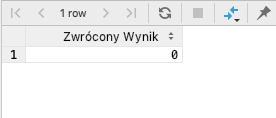
\includegraphics[width=0.25\textwidth]{procedura-utworz_uzytkownika-przyklad}
	\caption{Wynik prawidłowego uruchomienia przykładu użycia procedury \texttt{utworz\_uzytkownika}}
	\label{fig:lista_niepopularnych_obiektow}
\end{figure}

\begin{lstlisting}[language=SQL, caption={Przykład użycia procedury \texttt{utworz\_uzytkownika}}, label={lst:procedura-utworz_uzytkownika-przyklad}]
DECLARE @wynik INT;
EXEC @wynik = utworz_uzytkownika
  @login = 'j_kowalski',
  @nazwisko = 'Jan',
  @imie = 'Kowalski',
  @wiek = 25,
  @adres = 'Ul. Kowalska 23, 02-001, Warszawa',
  @telefon = '+48 625 548 874',
  @plec = 'M',
  @haslo = 'yourStrong(!)Password';
SELECT 'Zwrócony Wynik' = @wynik;
\end{lstlisting}

\subsubsection{\texttt{wynajmij\_obiekt} - Procedura do wynajmowania obiektów przez użytkowników}

Procedura ta służy do wynajmowania (tworzenia odpowiedniego wpisu w tabeli \texttt{najmy}) obiektów przez użytkowników.

Procedura przyjmuje 1 parametr:
\begin{itemize}
	\item `@obiekt_id INT`
\end{itemize}

Procedura zwraca następujące wartości:
\begin{itemize}
	\item 0 - Użytkownik dodany pomyślnie
	\item 1 - Wystąpił nieznany błąd
	\item 2 - Obiekt o podanym identyfikatorze nie istnieje
	\item 3 - Obiekt o podanym identyfikatorze jest obecnie zajęty
\end{itemize}

\begin{lstlisting}[language=SQL, caption={Skrypt tworzący procedurę składowaną \texttt{wynajmij\_obiekt}}, label={lst:procedura-wynajmij_obiekt}]
CREATE PROCEDURE wynajmij_obiekt
  @obiekt_id INT
  WITH EXECUTE AS OWNER
  AS
    IF NOT EXISTS(SELECT * FROM obiekty WHERE id = @obiekt_id)
      RETURN 2;

    IF EXISTS(SELECT * FROM obiekty WHERE id = @obiekt_id AND obecnie_wynajete = 't')
      RETURN 3;

    EXECUTE AS CALLER;
    DECLARE @login VARCHAR(75);
    SELECT @login = CURRENT_USER;
    REVERT;

    BEGIN TRANSACTION;
    INSERT INTO najmy (uzytkownik_id, obiekt_id, data_rozpoczecia, data_zakonczenia, koszt)
      VALUES ((SELECT u.id FROM dbo.uzytkownicy u WHERE u.login COLLATE SQL_Latin1_General_CP1_CS_AS = @login COLLATE SQL_Latin1_General_CP1_CS_AS), @obiekt_id, DEFAULT, NULL, NULL);

    IF @@ERROR<>0
      GOTO BLAD;

    COMMIT TRANSACTION;
    RETURN 0;

    BLAD:
      ROLLBACK TRANSACTION;
      RETURN 1;
\end{lstlisting}

\begin{lstlisting}[language=SQL, caption={Przykład użycia procedury \texttt{wynajmij\_obiekt}}, label={lst:procedura-wynajmij_obiekt-przyklad}]
DECLARE @wynik INT;
EXEC @wynik = wynajmij_obiekt @obiekt_id = 17;
SELECT 'Zwrócony Wynik' = @wynik;
\end{lstlisting}

\newpage

\subsection{Użytkownicy, role i uprawnienia}

Przewidziane zostały 3 role dla użytkowników:
\begin{itemize}
	\item \texttt{admini\_systemu} - Administratorzy - zarządzają obiektami, kategoriami i miastami
	\item \texttt{operatorzy\_systemu} - Operatorzy - zarządzają najmami (wynajem i zwroty)
	\item \texttt{uzytkownicy\_systemu} - Użytkownicy - zarządzają swoimi danymi oraz najmami
\end{itemize}
Do tych ról przypisane zostały uprawnienia zgodnie z tabelą \ref{table:permissions}.

Dodatkowo fabrycznie zostali utworzeni dwaj użytkownicy (listing \ref{lst:role-admin} i listing \ref{lst:role-operator}):
\begin{itemize}
	\item \texttt{admin} z hasłem \texttt{yourStrong(!)Password} przypisany do roli \texttt{admini\_systemu}
	\item \texttt{operator} z hasłem \texttt{yourStrong(!)Password} przypisany do roli \texttt{operatorzy\_systemu}
\end{itemize}

Kolejnych użytkowników roli \texttt{uzytkownicy\_systemu}, można tworzyć za pomocą procedury składowanej z listingu \ref{lst:procedura-utworz_uzytkownika-przyklad} - \texttt{utworz\_uzytkownika} (strona \ref{lst:procedura-utworz_uzytkownika-przyklad}).

\begin{table}[h]
	{\renewcommand{\arraystretch}{1.5}
		\begin{tabu} to \textwidth { |X[2,l]||X[1,c]|X[1,c]|X[1,c]| }
			\hline
			& \textbf{Administratorzy} & \textbf{Operatorzy} & \textbf{Użytkownicy} \\
			\hline
			\hline
			\multicolumn{4}{|c|}{\textbf{Tabele}} \\
			\hline
			\texttt{kategorie} & S, I, U, D & S & S \\
			\hline
			\texttt{miasta} & S, I, U, D & S & S \\
			\hline
			\texttt{dzielnice} & S, I, U, D & S & S \\
			\hline
			\texttt{obiekty} & S, I, U, D & S & S \\
			\hline
			\texttt{uzytkownicy} & S & S & S\footnotemark, U\footnotemark \\
			\hline
			\texttt{najmy} & S, I, U & S, I, U & S\footnotemark, U\footnotemark \\
			\hline
			\multicolumn{4}{|c|}{\textbf{Widoki}} \\
			\hline
			\texttt{lista\_najmow} & S & S & - \\
			\hline
			\texttt{lista\_niepopularnych\_obiektow} & S & - & - \\
			\hline
			\texttt{lista\_popularnosci\_obiektow} & S & - & - \\
			\hline
			\multicolumn{4}{|c|}{\textbf{Procedury}} \\
			\hline
			\texttt{utworz\_uzytkownika} & \multicolumn{3}{|c|}{tylko \texttt{dbo}} \\
			\hline
			\texttt{wynajmij\_obiekt} & - & - & X \\
			\hline
			\multicolumn{4}{|c|}{S - SELECT, I - INSERT, U - UPDATE, X - EXECUTE} \\
			\hline
		\end{tabu}
		\label{table:permissions}
		\caption{Role i ich uprawnienia}
	}
\end{table}

\addtocounter{footnote}{-4}
\stepcounter{footnote} \footnotetext{wybieranie i edycja ograniczone tylko do swoich danych}
\stepcounter{footnote} \footnotetext{tylko pola nazwisko, imie, wiek, adres, telefon, plec}
\stepcounter{footnote} \footnotetext{wybieranie i edycja ograniczone tylko do swoich danych}
\stepcounter{footnote} \footnotetext{tylko pole data\_zakonczenia}

\begin{lstlisting}[language=SQL, caption={Skrypt tworzący rolę i użytkownika administracyjnego}, label={lst:role-admin}]
CREATE ROLE admini_systemu;
GO;

GRANT SELECT, INSERT, UPDATE, DELETE ON kategorie TO admini_systemu;
GO;

GRANT SELECT, INSERT, UPDATE, DELETE ON miasta TO admini_systemu;
GO;

GRANT SELECT, INSERT, UPDATE, DELETE ON dzielnice TO admini_systemu;
GO;

GRANT SELECT, INSERT, UPDATE, DELETE ON obiekty TO admini_systemu;
GO;

GRANT SELECT, UPDATE, DELETE ON uzytkownicy TO admini_systemu;
GO;

GRANT SELECT, INSERT, UPDATE ON najmy TO admini_systemu;
GO;

GRANT SELECT ON lista_najmow TO admini_systemu;
GO;

GRANT SELECT ON lista_niepopularnych_obiektow TO admini_systemu;
GO;

GRANT SELECT ON lista_popularnosci_obiektow TO admini_systemu;
GO;

CREATE USER admin WITH PASSWORD ='yourStrong(!)Password';
GO;

EXEC sp_addrolemember 'admini_systemu', 'admin';
GO;
\end{lstlisting}

\begin{lstlisting}[language=SQL, caption={Skrypt tworzący rolę i użytkownika operatorskiego}, label={lst:role-operator}]
CREATE ROLE operatorzy_systemu;
GO;

GRANT SELECT ON kategorie TO operatorzy_systemu;
GO;

GRANT SELECT ON miasta TO operatorzy_systemu;
GO;

GRANT SELECT ON dzielnice TO operatorzy_systemu;
GO;

GRANT SELECT ON obiekty TO operatorzy_systemu;
GO;

GRANT SELECT ON uzytkownicy TO operatorzy_systemu;
GO;

GRANT SELECT, INSERT, UPDATE ON najmy TO operatorzy_systemu;
GO;

GRANT SELECT ON lista_najmow TO operatorzy_systemu;
GO;

CREATE USER operator WITH PASSWORD ='yourStrong(!)Password';
GO;

EXEC sp_addrolemember 'operatorzy_systemu', 'operator';
GO;
\end{lstlisting}

\subsubsection{Ograniczenie uprawnień na poziomie wiersza}

\textbf{Uwaga:} Funkcjonalność \href{https://docs.microsoft.com/en-us/sql/relational-databases/security/row-level-security?view=sql-server-2017}{Row Level Security (RLS)} została wprowadzona w SQL Server 2016. Próba uruchomienia tych skryptów na wersji niższej niż 2016 skończy się niepowodzeniem.

W tabelach \texttt{uzytkownicy} oraz \texttt{najmy} została ograniczona widoczność grupie \texttt{uzytkownicy\_systemu} tylko do rekordów powiązanych z zalogowanym użytkownikiem. Jest to możliwe dzięki funkcjonalności \href{https://docs.microsoft.com/en-us/sql/relational-databases/security/row-level-security?view=sql-server-2017}{Row Level Security}. Sposób utworzenia ograniczenia RLS można zobaczyć na listingu \ref{lst:rls-uzytkownicy} oraz listingu \ref{lst:rls-najmy}.

\begin{lstlisting}[language=SQL, caption={Skrypt ustawiający ograniczenie RLS na tabeli \texttt{uzytkownicy}}, label={lst:rls-uzytkownicy}]
CREATE FUNCTION fn_securitypredicate_uzytkownicy (@login_field SYSNAME)
  RETURNS TABLE
  WITH SCHEMABINDING
  AS
    RETURN SELECT 1 AS fn_securitypredicate_uzytkownicy_result
      FROM dbo.uzytkownicy
      WHERE (
        @login_field = user_name()
        OR IS_ROLEMEMBER('admini_systemu', user_name()) = 1
        OR IS_ROLEMEMBER('operatorzy_systemu', user_name()) = 1
        OR user_name() = 'dbo'
      )
GO;

CREATE SECURITY POLICY fn_security_uzytkownicy
  ADD FILTER PREDICATE
  dbo.fn_securitypredicate_uzytkownicy(login)
  ON dbo.uzytkownicy
GO;

ALTER SECURITY POLICY fn_security_uzytkownicy WITH (state = on);
GO;
\end{lstlisting}

\begin{lstlisting}[language=SQL, caption={Skrypt ustawiający ograniczenie RLS na tabeli \texttt{najmy}}, label={lst:rls-najmy}]
CREATE FUNCTION fn_securitypredicate_najmy (@login_field SYSNAME)
  RETURNS TABLE
  WITH SCHEMABINDING
  AS
    RETURN SELECT 1 AS fn_securitypredicate_najmy_result
      FROM dbo.najmy n
      WHERE (
        @login_field = (SELECT u.id FROM dbo.uzytkownicy u WHERE u.login COLLATE SQL_Latin1_General_CP1_CS_AS = CURRENT_USER COLLATE SQL_Latin1_General_CP1_CS_AS)
        OR IS_ROLEMEMBER('admini_systemu', user_name()) = 1
        OR IS_ROLEMEMBER('operatorzy_systemu', user_name()) = 1
        OR user_name() = 'dbo'
      )
GO;

CREATE SECURITY POLICY fn_security_najmy
  ADD FILTER PREDICATE
  dbo.fn_securitypredicate_najmy(uzytkownik_id)
  ON dbo.najmy
GO;

ALTER SECURITY POLICY fn_security_najmy WITH (state = on);
GO;
\end{lstlisting}

\subsubsection{Test uprawnień użytkowników}

W pierwszy teście sprawdzimy czy do widoku \texttt{lista\_najmow}, uprawnienia mają tylko użytkownicy grup \texttt{operatorzy\_systemu} oraz \texttt{admini\_systemu}.

\lstinputlisting[language=SQL, caption={Skrypt testujący uprawnienia do wyświetlania widoku \texttt{lista\_najmow}}, label={lst:test-lista_najmow}]{../DockerMachine/MSSQLServer/scripts/test-lista_najmow.sql}

\lstinputlisting[caption={Wynik uruchomienia skryptu testującego uprawnienia do wyświetlania widoku \texttt{lista\_najmow}}, label={lst:test-lista_najmow-results}]{../Logs/test-lista_najmow.sql.log}

W drugim teście sprawdzimy czy \texttt{uzytkownicy\_systemu} widzą tylko swoje dane w tabeli \texttt{uzytkownicy}, a \texttt{operatorzy\_systemu} oraz \texttt{admini\_systemu} widzą wszystkich 4 użytkowników.

\lstinputlisting[language=SQL, caption={Skrypt testujący uprawnienia do wyświetlania tabeli \texttt{uzytkownicy}}, label={lst:test-uzytkownicy}]{../DockerMachine/MSSQLServer/scripts/test-uzytkownicy.sql}

\lstinputlisting[caption={Wynik uruchomienia skryptu testującego uprawnienia do wyświetlania tabeli \texttt{uzytkownicy}}, label={lst:test-uzytkownicy-results}]{../Logs/test-uzytkownicy.sql.log}

\section{Skrypt tworzący dane testowe}

ZRZUT EKRANÓW Z KOMUNIKATÓW PO WSTAWIANIU DANYCH <np. ILE DANYCH
DO KAZDEJ TABELI WPROWADZONO>

\section{Skrypt tworzący użytkowników i nadający uprawnienia}

% TODO: Uzupełnić

8. SKRYPT TWORZĄCY UŻYTKOWNIKÓW BAZY DANYCH <KONTA, UPRAWNIENIA itp>
W FORMIE:
a. OPIS UŻYTKOWNIKÓW <ICH ZADANIA>
b. SKŁADNIA SKRYPTU
c. ZRZUTY EKRANU Z: UTWORZENIA UZYTKOWNIKÓW, UPRAWNIENIA, TEST
MOZLIWOŚCI/NIE MOZLIWOŚCI KAZDEGO Z NICH

\section{Skrypt usuwający obiekty z bazy danych}

\subsection{Wynik uruchomienia całego skryptu w trybie wsadowym}

Jak widać na listingu \ref{lst:destroy-objects}, skrypt podaje bardzo dokładne informacje na temat aktualnie wykonywanej operacji. W przypadku tego skryptu, operacje są wykonywane w odwrotnej kolejności niż w skrypcie tworzącym z listingu \ref{lst:create-objects}.

\lstinputlisting[caption=Wynik uruchomienia całego skryptu usuwającego w trybie wsadowym, label={lst:destroy-objects}]{../Logs/skrypt_usuwajacy_obiekty_z_bazy.sql.log}

\section{Skrypt usuwający użytkowników i uprawnienia}
% TODO: Uzupełnić

\section{Skrypt usuwający dane testowe}

Ponieważ nasze tabele posiadają kolumny autonumerowanie (typu \texttt{IDENTITY}), to nie możemy skasować danych przy pomocy funkcji \texttt{TRUNCATE}. Aby uzyskać podobny wynik (opróżnienie tabeli ) wykorzystuję dyrektywę \texttt{DBCCCHECKIDENT(<tabela>, RESEED, 0)} która powoduje zresetowanie autonumerowania.

\lstinputlisting[language=SQL, caption=Skrypt usuwający dane testowe, label={lst:destroy-data-script}]{../../skrypt_usuwajacy_dane_testowe.sql}

\subsection{Wynik uruchomienia całego skryptu w trybie wsadowym}

\lstinputlisting[caption=Wynik uruchomienia całego skryptu usuwającego dane testowe w trybie wsadowym, label={lst:destroy-data}]{../Logs/skrypt_usuwajacy_dane_testowe.sql.log}







\section{Przykłady kodu LaTeX}
Projekt systemu\footnote{footnotes working fine} zawiera założenia do bazy danych przechowującej informacje\footnote{footnotes working fine} potrzebne

\subsection{Tytuł podrozdziału} 
\subsubsection{Tytuł podpodrozdziału}
\textbf{Pogrubiony tekst}
\texttt{treść pisma technicznego}
\textsl{tekst do pochylenia}
\href{http://www.sharelatex.com}{Something 
Linky}
 
\begin{itemize}
\item pierwszy element
\item drugi element
\item trzeci element...
\end{itemize}

\subsubsection{Tytuł podpodrozdziału 2}
\begin{enumerate}
\item pierwszy element
\item drugi element
\item trzeci element...
\end{enumerate}

\lstinputlisting[language=SQL, caption=skrypt\_tworzacy\_obiekty\_w\_bazie\_danych.sql]{../../skrypt_tworzacy_obiekty_w_bazie_danych.sql}


\lstinputlisting[language=SQL,caption=skrypt\_usuwajacy\_obiekty\_z\_bazy.sql.sql]{../../skrypt_usuwajacy_obiekty_z_bazy.sql}



\lstlistoflistings
\listoffigures

\end{document}
